\subsection{Man in the Middle (MITM)}

\subsubsection{Tấn công MITM là gì?}
    Cuộc tấn công giữa chừng (MITM) là một thuật ngữ chung khi thủ phạm tự đặt mình vào cuộc trò chuyện giữa người dùng và ứng dụng để nghe trộm hoặc mạo danh một trong các bên hoặc cũng có thể chặn lưu lượng truy cập thậm chí có thể chặn liên lạc giữa hai máy, khiến cuộc trò chuyện có vẻ như là một cuộc trao đổi thông tin bình thường đang được tiến hành.
    
Mục tiêu của cuộc tấn công là đánh cắp thông tin cá nhân, chẳng hạn như thông tin đăng nhập, chi tiết tài khoản và số thẻ tín dụng. Mục tiêu thường là người dùng các ứng dụng tài chính, doanh nghiệp SaaS, trang web thương mại điện tử và các trang web khác yêu cầu đăng nhập.

Thông tin thu được trong một cuộc tấn công có thể được sử dụng cho nhiều mục đích, bao gồm đánh cắp danh tính, chuyển tiền không được phê duyệt hoặc thay đổi mật khẩu bất hợp pháp.

Ngoài ra, nó có thể được sử dụng để giành được chỗ đứng bên trong vành đai an toàn trong giai đoạn xâm nhập của một  cuộc tấn công có mối đe dọa dai dẳng  (APT) nâng cao.
\begin{figure}[H]
    \centering
    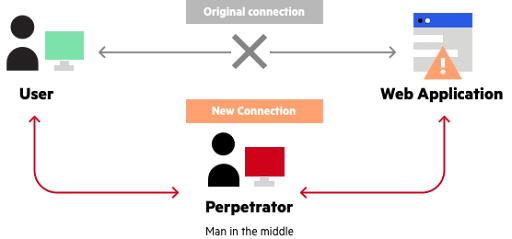
\includegraphics[scale=0.7]{pic/huê/mitm.png}
    
    \caption{Tấn công MITM}
\end{figure}
Nói rộng hơn, một cuộc tấn công MITM tương đương với việc một người đưa thư mở bảng sao kê ngân hàng của bạn, viết chi tiết tài khoản của bạn rồi dán lại phong bì và chuyển nó đến tận nhà bạn.
\subsubsection{Các kiểu tấn công MITM}
Cuộc tấn công trung gian trong an ninh mạng được coi là bất kỳ trường hợp nào mà tác nhân đe dọa đặt mình vào giữa người dùng và một thực thể như mạng, trang web hoặc ứng dụng để lấy thông tin. Phương pháp mà tin tặc lấy được thông tin đó khác nhau bằng cách sử dụng các hình thức giả mạo khác nhau, một phương pháp mạo danh các thực thể hoặc trang web trực tuyến đáng tin cậy. Các loại tấn công MITM chính bao gồm:
\begin{itemize}
    \item Giả mạo IP: Tội phạm mạng thay đổi địa chỉ Giao thức Internet (IP) của trang web, địa chỉ email hoặc thiết bị và giả mạo thực thể—khiến người dùng nghĩ rằng họ đang tương tác với một nguồn đáng tin cậy trong khi họ thực sự đang chuyển thông tin cho một tác nhân độc hại.
    \item Giả mạo DNS: Đối với giả mạo Hệ thống tên miền (DNS), kẻ gửi thư rác tạo và vận hành một trang web giả mạo mà người dùng quen thuộc và định tuyến chúng đến trang web đó để lấy thông tin xác thực của người dùng hoặc thông tin khác.
    \item Giả mạo HTTPS: Người dùng cho rằng một trang web có Bảo mật Giao thức Truyền Siêu Văn bản (HTTPS), nghĩa là họ đã mã hóa dữ liệu máy tính của mình vào máy chủ lưu trữ trang web. Tuy nhiên, chúng đã được bí mật chuyển hướng đến một trang web HTTP không an toàn, cho phép bọn tội phạm theo dõi các tương tác và đánh cắp thông tin.
\item Chiếm đoạt email: Những kẻ tấn công bí mật truy cập vào tài khoản email của ngân hàng hoặc công ty phát hành thẻ tín dụng để theo dõi các giao dịch và đánh cắp thông tin. Họ cũng có thể sử dụng tài khoản email hoặc địa chỉ email giả mạo hơi khác so với địa chỉ thực tế để cung cấp hướng dẫn sai cho khách hàng, chẳng hạn như chuyển tiền vào tài khoản séc mới.
\item Wifi Eavesdropping: Người gửi thư rác tạo các mạng Wi-Fi công cộng hoặc các điểm phát sóng có vẻ như là một doanh nghiệp lân cận hoặc nguồn đáng tin cậy khác. Người dùng kết nối sau đó sẽ bị chặn tất cả hoạt động và dữ liệu nhạy cảm của họ.
\item Tấn công SSL: Một phần mở rộng của hoạt động giả mạo HTTPS, chiếm quyền điều khiển Lớp cổng bảo mật (SSL) là khi tin tặc lấy giao thức này chịu trách nhiệm mã hóa các kết nối HTTPS và chặn dữ liệu người dùng di chuyển giữa họ và máy chủ mà họ đang kết nối.
\item Chiếm quyền điều khiển phiên: Thường được gọi là hành vi trộm cắp cookie trình duyệt, kẻ tấn công sẽ đánh cắp thông tin được lưu trữ trên cookie trình duyệt web, chẳng hạn như mật khẩu đã lưu.
\end{itemize}
\subsubsection{Tiến trình tấn công MITM}
Việc thực thi MITM thành công có hai giai đoạn riêng biệt: Chặn và Giải mã.
\begin{itemize}
    \item Chặn:\\
    Bước đầu tiên chặn lưu lượng truy cập của người dùng qua mạng của kẻ tấn công trước khi nó đến đích dự định.
    
Cách phổ biến nhất (và đơn giản nhất) để thực hiện việc này là tấn công thụ động, trong đó kẻ tấn công cung cấp các điểm truy cập WiFi độc hại, miễn phí cho công chúng. Thường được đặt tên theo cách tương ứng với vị trí của chúng, chúng không được bảo vệ bằng mật khẩu. Khi nạn nhân kết nối với một điểm phát sóng như vậy, kẻ tấn công sẽ có được khả năng hiển thị đầy đủ đối với bất kỳ hoạt động trao đổi dữ liệu trực tuyến nào.

Những kẻ tấn công muốn thực hiện một cách tiếp cận tích cực hơn để đánh chặn có thể thực hiện một trong các cuộc tấn công sau:
\begin{itemize}
    \item Giả mạo IP  liên quan đến kẻ tấn công cải trang thành một ứng dụng bằng cách thay đổi tiêu đề gói trong địa chỉ IP. Kết quả là người dùng cố gắng truy cập URL được kết nối với ứng dụng sẽ được gửi đến trang web của kẻ tấn công.
    \item Giả mạo ARP  là quá trình liên kết địa chỉ MAC của kẻ tấn công với địa chỉ IP của người dùng hợp pháp trên mạng cục bộ bằng cách sử dụng tin nhắn ARP giả mạo. Do đó, dữ liệu do người dùng gửi đến địa chỉ IP máy chủ thay vào đó sẽ được truyền đến kẻ tấn công.

\item Giả mạo DNS , còn được gọi là đầu độc bộ đệm DNS, liên quan đến việc xâm nhập vào máy chủ DNS và thay đổi bản ghi địa chỉ của trang web. Kết quả là, người dùng cố gắng truy cập trang web sẽ được bản ghi DNS đã thay đổi gửi đến trang web của kẻ tấn công.

\end{itemize}
\item Giải mã:\\
Sau khi chặn, mọi lưu lượng SSL hai chiều cần được giải mã mà không thông báo cho người dùng hoặc ứng dụng. Một số phương pháp tồn tại để đạt được điều này:
\begin{itemize}
    \item Việc giả mạo HTTPS  gửi chứng chỉ giả mạo đến trình duyệt của nạn nhân sau khi yêu cầu kết nối ban đầu tới một trang web an toàn được thực hiện. Nó chứa dấu vân tay kỹ thuật số liên quan đến ứng dụng bị xâm nhập mà trình duyệt sẽ xác minh theo danh sách các trang web đáng tin cậy hiện có. Kẻ tấn công sau đó có thể truy cập bất kỳ dữ liệu nào do nạn nhân nhập trước khi nó được chuyển đến ứng dụng.

\item SSL BEAST  (khai thác trình duyệt chống lại SSL/TLS) nhắm vào lỗ hổng TLS phiên bản 1.0 trong SSL. Tại đây, máy tính của nạn nhân bị nhiễm JavaScript độc hại có chức năng chặn các cookie được mã hóa được gửi bởi một ứng dụng web. Sau đó, chuỗi khối mật mã (CBC) của ứng dụng bị xâm phạm để giải mã cookie và mã thông báo xác thực của ứng dụng.

\item Việc chiếm quyền điều khiển SSL  xảy ra khi kẻ tấn công chuyển các khóa xác thực giả mạo cho cả người dùng và ứng dụng trong quá trình bắt tay TCP. Điều này thiết lập những gì có vẻ là một kết nối an toàn trong khi trên thực tế, người đàn ông ở giữa kiểm soát toàn bộ phiên.
\item  Việc loại bỏ SSL  hạ cấp kết nối HTTPS xuống HTTP bằng cách chặn xác thực TLS được gửi từ ứng dụng tới người dùng. Kẻ tấn công gửi phiên bản không được mã hóa của trang web ứng dụng cho người dùng trong khi vẫn duy trì phiên bảo mật với ứng dụng. Trong khi đó, kẻ tấn công có thể nhìn thấy toàn bộ phiên của người dùng.
\end{itemize}
\end{itemize}
\subsubsection{Mức độ phổ biến của các cuộc tấn công Man-In-The-Middle}
Các cuộc tấn công MITM rất phổ biến, mặc dù không đến mức Ransomware hoặc lừa đảo. Các kiểu tấn công này rất dễ thực hiện và các công cụ hack được cung cấp công khai. Chúng được thực hiện không chỉ từ bên ngoài, mà còn có những sự cố bên trong tổ chức nơi MITM được sử dụng để tấn công mạng nội bộ.
\newline
Thật không may, những loại sự cố này rất khó phát hiện, đó là lý do tại sao hành động ngăn chặn là rất quan trọng, đồng thời cũng giúp cải thiện an ninh mạng và quyền riêng tư.

\subsubsection{Các công cụ được sử dụng }
\begin{itemize}
    \item \textbf{Windows}: Ví dụ, Cain và Abel – không sử dụng, nhưng nó có vẻ là một công cụ mạnh mẽ để lấy mật khẩu trên mạng.
    \item \textbf{Android}: cSploit. Là một ứng dụng mã nguồn mở được phát triển cho điện thoại Android. Để bắt đầu chạy nó, bạn phải có đặc quyền root trên điện thoại của mình. Nó yêu cầu cho phép rất nhiều và hoạt động của nó chỉ đơn giản là chọn từ menu những gì chúng ta muốn làm – thay thế hình ảnh, kiểm tra lưu lượng mạng hoặc giải mã các gói đã gửi.
    \item \textbf{Linux}: Kali Linux là một bản phân phối Linux dành cho tin tặc.
\end{itemize}
\subsubsection{Biện pháp bảo vệ và ngăn chặn}
\begin{figure}[H]
    \centering
    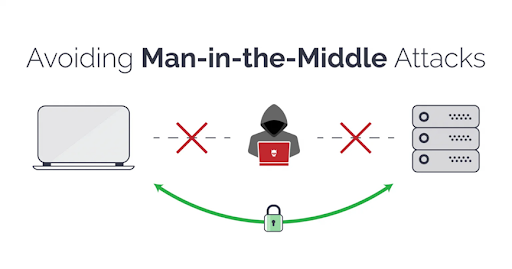
\includegraphics[scale=0.8]{pic/huê/tấn công mitm.png}
    
    \caption{Bảo vệ và ngăn chặn tấn công MITM}
\end{figure}
Việc ngăn chặn tấn công MITM yêu cầu một số bước nhất định từ người dùng. Cùng với đó là kết hợp các phương thức mã hóa và xác minh khác. Do đó để bảo vệ và ngăn chặn tấn công cần có sự kết hợp giữa người dùng và quản trị viên:
\begin{itemize}
    \item  Đối với người dùng:

\begin{itemize}
    \item Tránh các kết nối WiFi không được bảo vệ bằng password, vì chúng dễ bị tấn công và bị tội phạm mạng đánh cắp dữ liệu.
    \item Chú ý đến các thông báo của trình duyệt về trang web không an toàn.\cite{ylli2021man}
\item Đăng xuất khỏi các ứng dụng không không sử dụng nữa.
\item  Không sử dụng mạng công cộng (ở quán cafe, cửa hàng, khách sạn…) khi thực hiện các giao dịch nhạy cảm.

\item  Tránh email lừa đảo: Tội phạm mạng thường tạo ra các email lừa đảo để lừa người dùng mở chúng. Người dùng cần cân nhắc kỹ trước khi mở email đến từ nguồn không xác minh hoặc không rõ. Thông thường, email lừa đảo sẽ giả mạo một nguồn đáng tin cậy, như một tài khoản ngân hàng hoặc một tổ chức tài chính. Những email này thường yêu cầu người dùng nhấp vào liên kết để nhập thông tin đăng nhập hoặc cập nhật mật khẩu. Tuyệt đối tránh nhấp vào các liên kết này, vì chúng có thể chuyển hướng người dùng đến trang web giả mạo hoặc tải xuống phần mềm độc hại \cite{ylli2021man}.
\end{itemize}
\item  Đối với quản trị viên:
\begin{itemize}
    \item Tạo kết nối bảo mật: Bước đầu tiên để chống lại các cuộc tấn công MitM là đảm bảo kết nối an toàn. Người dùng chỉ nên truy cập các trang web hiển thị “HTTPS” trong thanh địa chỉ URL, thay vì chỉ “HTTP”. Hầu hết các trình duyệt web hiển thị biểu tượng ổ khóa trước URL để chỉ ra rằng trang web là an toàn. Việc này sẽ giúp giảm thiểu tấn công giả mạo bằng cách mã hóa và xác thực dữ liệu. Quản trị viên nên áp dụng việc xác thực đa yếu tố cho tất cả người dùng, để tăng cường thêm một lớp bảo mật cho việc truyền thông trực tuyến \cite{ylli2021man}.
\item Sử dụng mã hóa mạng riêng ảo (VPN): VPN mã hóa kết nối internet và truyền dữ liệu trực tuyến như mật khẩu và thông tin thẻ tín dụng, và nên được sử dụng khi kết nối đến các mạng Wi-Fi công cộng và điểm phát sóng không an toàn. VPN có thể ngăn chặn tiềm năng các cuộc tấn công MitM. Ngay cả khi tội phạm mạng có thể truy cập vào mạng, họ cũng sẽ không thể giải mã các tin nhắn hoặc truy cập tài nguyên do mã hóa bởi VPN cung cấp. Tổ chức cũng cần đảm bảo nhân viên đăng nhập hệ thống qua mạng riêng ảo của công ty, đặc biệt khi làm việc từ xa \cite{ylli2021man}.
\item  Bảo vệ điểm cuối: Triển khai bảo mật điểm cuối toàn diện là rất quan trọng khi cố gắng ngăn chặn sự lan truyền của phần mềm độc hại và các cuộc tấn công mạng khác. Vì các cuộc tấn công MitM thường sử dụng phần mềm độc hại để thực hiện, việc cài đặt sản phẩm chống phần mềm độc hại và bảo mật internet là hết sức quan trọng.
\end{itemize}
\end{itemize}
\subsection{Tấn công Kết hợp Plaintext-Ciphertext (Known- Plaintext Attack)
}
\subsubsection{Know-Plaintext Attack là gì?}
Known-plaintext attacks (KPA) là khi tin tặc sử dụng bản rõ và bản mã để xác định thuật toán hoặc khóa mã hóa.

Trong một Known-plaintext Attacks, kẻ tấn công có quyền truy cập vào cả dạng mã hóa của dữ liệu (ciphertext) và bản sao văn bản gốc tương ứng của dữ liệu gốc (unencrypted form). Kẻ tấn công cố gắng xác định khóa hoặc thuật toán mã hóa bằng cách kiểm tra mối quan hệ giữa plaintext và ciphertext.

Ví dụ: nếu “CRYPTO” được mã hóa thành “XUZZA”, việc biết cặp này có thể cho phép kẻ tấn công giải mã các phần khác của tin nhắn cũng được mã hóa bằng cùng một khóa thay thế. Điều này chứng tỏ rằng, với một số thuật toán mã hóa, ngay cả một lượng kiến thức nhỏ cũng có thể dẫn đến việc giải mã rộng hơn.

Kiểu tấn công này sử dụng một lỗ hổng trong kỹ thuật mã hóa giúp xác định các mẫu hoặc kết nối được tạo ra giữa bản rõ và bản mã. Nếu không được ngăn chặn một cách chính xác, các Known-plaintext Attacks có thể gây nguy hiểm cho tính bảo mật của hệ thống mã hóa.

Hai phương pháp phổ biến để khai thác plaintext và dạng mã hóa tương ứng của nó nhằm khám phá các khóa mã hóa bao gồm phân tích tần số (frequency analysis) và khớp mẫu (pattern matching). Phương pháp phân tích tần số sử dụng các phương pháp mã hóa đơn giản bằng cách thay thế từng ký tự hoặc ký hiệu một-một. Những kẻ tấn công có thể tìm ra chìa khóa hoặc mở khóa phần còn lại của giao tiếp bằng cách so sánh tần suất xuất hiện của các chữ cái hoặc mẫu cụ thể trong plaintext và bản mã liên quan.

Những kẻ tấn công có thể phát hiện ra các xu hướng khi cùng một plaintext tạo ra cùng một bản mã theo phương pháp khớp mẫu. Họ có thể nhận ra thuật toán mã hóa và giải mã toàn bộ tin nhắn bằng cách xác định các mẫu trong văn bản được mã hóa và so sánh chúng với các mẫu đã biết trong plaintext gốc.

\begin{figure}[H]
    \centering
    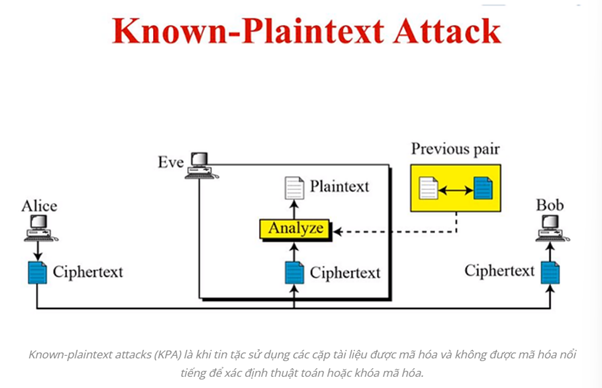
\includegraphics[scale=0.9]{pic/huê/kpa.png}
    
    \caption{Tấn công Know-Plaintext}
\end{figure}
\subsubsection{KPA đã hoạt động như nào?
}
Trong KPA, kẻ tấn công có thể tìm hiểu các chi tiết quan trọng về phương pháp mã hóa bằng cách phân tích cách các đoạn cụ thể của văn bản gốc được chuyển đổi thành văn bản mã hóa bằng cách sử dụng cùng một khóa hoặc thuật toán mã hóa.

Cuộc tấn công bao gồm các bước sau:
\begin{itemize}
    \item \textbf{Thu thập các cặp đã biết:}
Kẻ tấn công tích lũy các cặp plaintext và văn bản mật mã được mã hóa liên quan có được thông qua các kỹ thuật khác nhau, chẳng hạn như thông tin liên lạc bị chặn hoặc rò rỉ dữ liệu.
\item \textbf{Phân tích mẫu:}
Khi bản rõ được mã hóa để tạo thành bản mã, kẻ tấn công sẽ so sánh các mẫu, sửa đổi và biến đổi diễn ra. Để hiểu hoạt động của quá trình mã hóa, họ tìm kiếm các mối quan hệ thường xuyên giữa plaintext và ciphertext đã biết.
\item \textbf{Lấy khóa hoặc thuật toán:}
Kẻ tấn công cố gắng xác định các yếu tố mã hóa quan trọng, chẳng hạn như khóa mã hóa, thuật toán hoặc các tham số quy trình khác, dựa trên các mẫu mà chúng đã nhận thấy. Họ có thể sao chép độc lập quá trình mã hóa nhờ vào suy luận này.
\item \textbf{Giải mã dữ liệu khác:}
Kẻ tấn công có thể giải mã các tài liệu được mã hóa khác sử dụng cùng một thuật toán mã hóa bằng cách sử dụng khóa hoặc thuật toán được suy luận. Quy trình này có thể làm rò rỉ thông tin bí mật hoặc gây nguy hiểm cho tính bảo mật của hệ thống mã hóa.

\end{itemize}
\subsubsection{Biện pháp bảo vệ và ngăn chặn}
Để bảo vệ chống lại các Known-plaintext Attacks, hãy áp dụng thuật toán mã hóa mạnh, quản lý khóa mã hóa một cách an toàn, sử dụng khóa duy nhất cho mỗi phiên và thêm tính ngẫu nhiên vào quy trình mã hóa để tăng cường khả năng bảo vệ chống lại các cuộc tấn công.
\begin{itemize}
    \item \textbf{Áp dụng thuật toán mã hóa mạnh:} Bằng cách ngăn chặn các mẫu trong bản rõ tương quan với các mẫu trong văn bản mã hóa, các thuật toán mã hóa hiện đại như Tiêu chuẩn mã hóa nâng cao (AES) được tạo ra để tồn tại trước các cuộc tấn công như vậy. AES là một thuật toán mã hóa đối xứng được sử dụng rộng rãi, nổi tiếng về tính bảo mật và hiệu quả.
\item \textbf{Quản lý an toàn các khóa mã hóa:} Bằng cách quản lý an toàn  ta có thể  tránh truy cập trái phép. Sử dụng kho lưu trữ khóa an toàn, xoay khóa thường xuyên và sử dụng các kỹ thuật tạo khóa mạnh mẽ. Ngoài ra, tránh mã hóa các khối dữ liệu rời rạc, có thể dự đoán được. Để ngăn kẻ tấn công sử dụng các cặp đã biết, hãy mã hóa toàn bộ tin nhắn hoặc tệp.
\item \textbf{Sử dụng khóa duy nhất cho mỗi phiên:} sử dụng các phím khác nhau cho các phiên và nỗ lực khác nhau. Tác động của Known-plaintext Attacks đã giảm do mỗi phiên sẽ sử dụng một khóa mã hóa khác nhau. Ngoài ra, hãy duy trì các phiên bản mới nhất của hệ thống, thư viện và phần mềm mã hóa của bạn. Các bản sửa lỗi bảo mật giúp sửa chữa các lỗ hổng thường được đưa vào các bản cập nhật.
\item  \textbf{Thêm tính ngẫu nhiên vào quy trình mã hóa:} Trước khi mã hóa bản rõ của dữ liệu, hãy thêm một giá trị ngẫu nhiên vào đó. Điều này làm cho mỗi mã hóa là duy nhất, ngay cả khi mã hóa cùng một bản rõ nhiều lần. Ngoài ra, hãy tránh các phương pháp mã hóa được biết là dễ bị tấn công bằng plaintext đã biết. Điều đó nói rằng, hãy thực hiện thẩm định thích hợp khi chọn thuật toán mã hóa.

\end{itemize}